\section{Structure du site et style}

Dans un premier temps, nous avons créé des premières pages HTML afin d'avoir un rendu visuel.
Elles devaient être responsive grâce à Bootstrap et permettre de définir un style CSS servant à voir, pour le développement, à quoi s'apparenterait les pages finales.

\begin{figure}[H]
    \begin{center}
	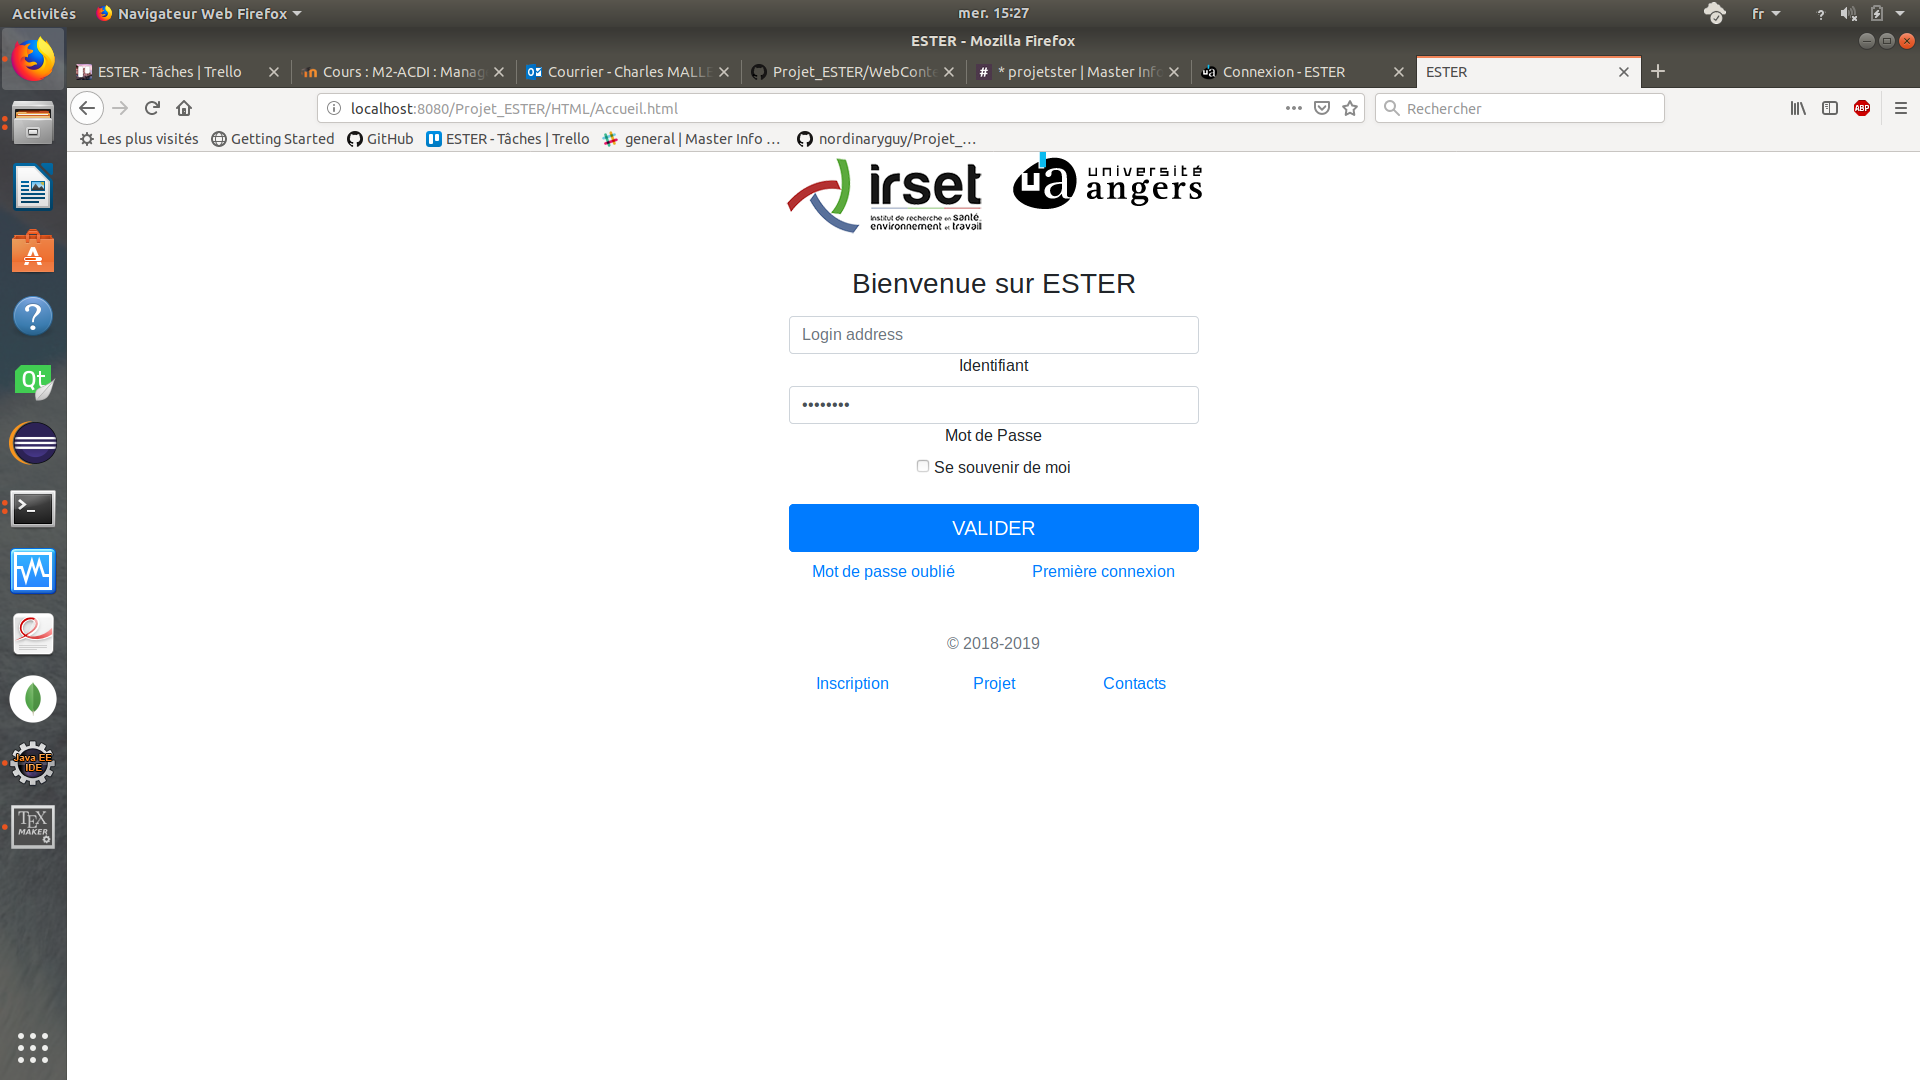
\includegraphics[scale=0.2,trim=4cm 0cm 4cm 5.3cm, clip=true]{img/OldConnexion}
    \end{center}
    \caption{Ancienne Page de Connexion}
\end{figure}

\begin{figure}[H]
    \begin{center}
	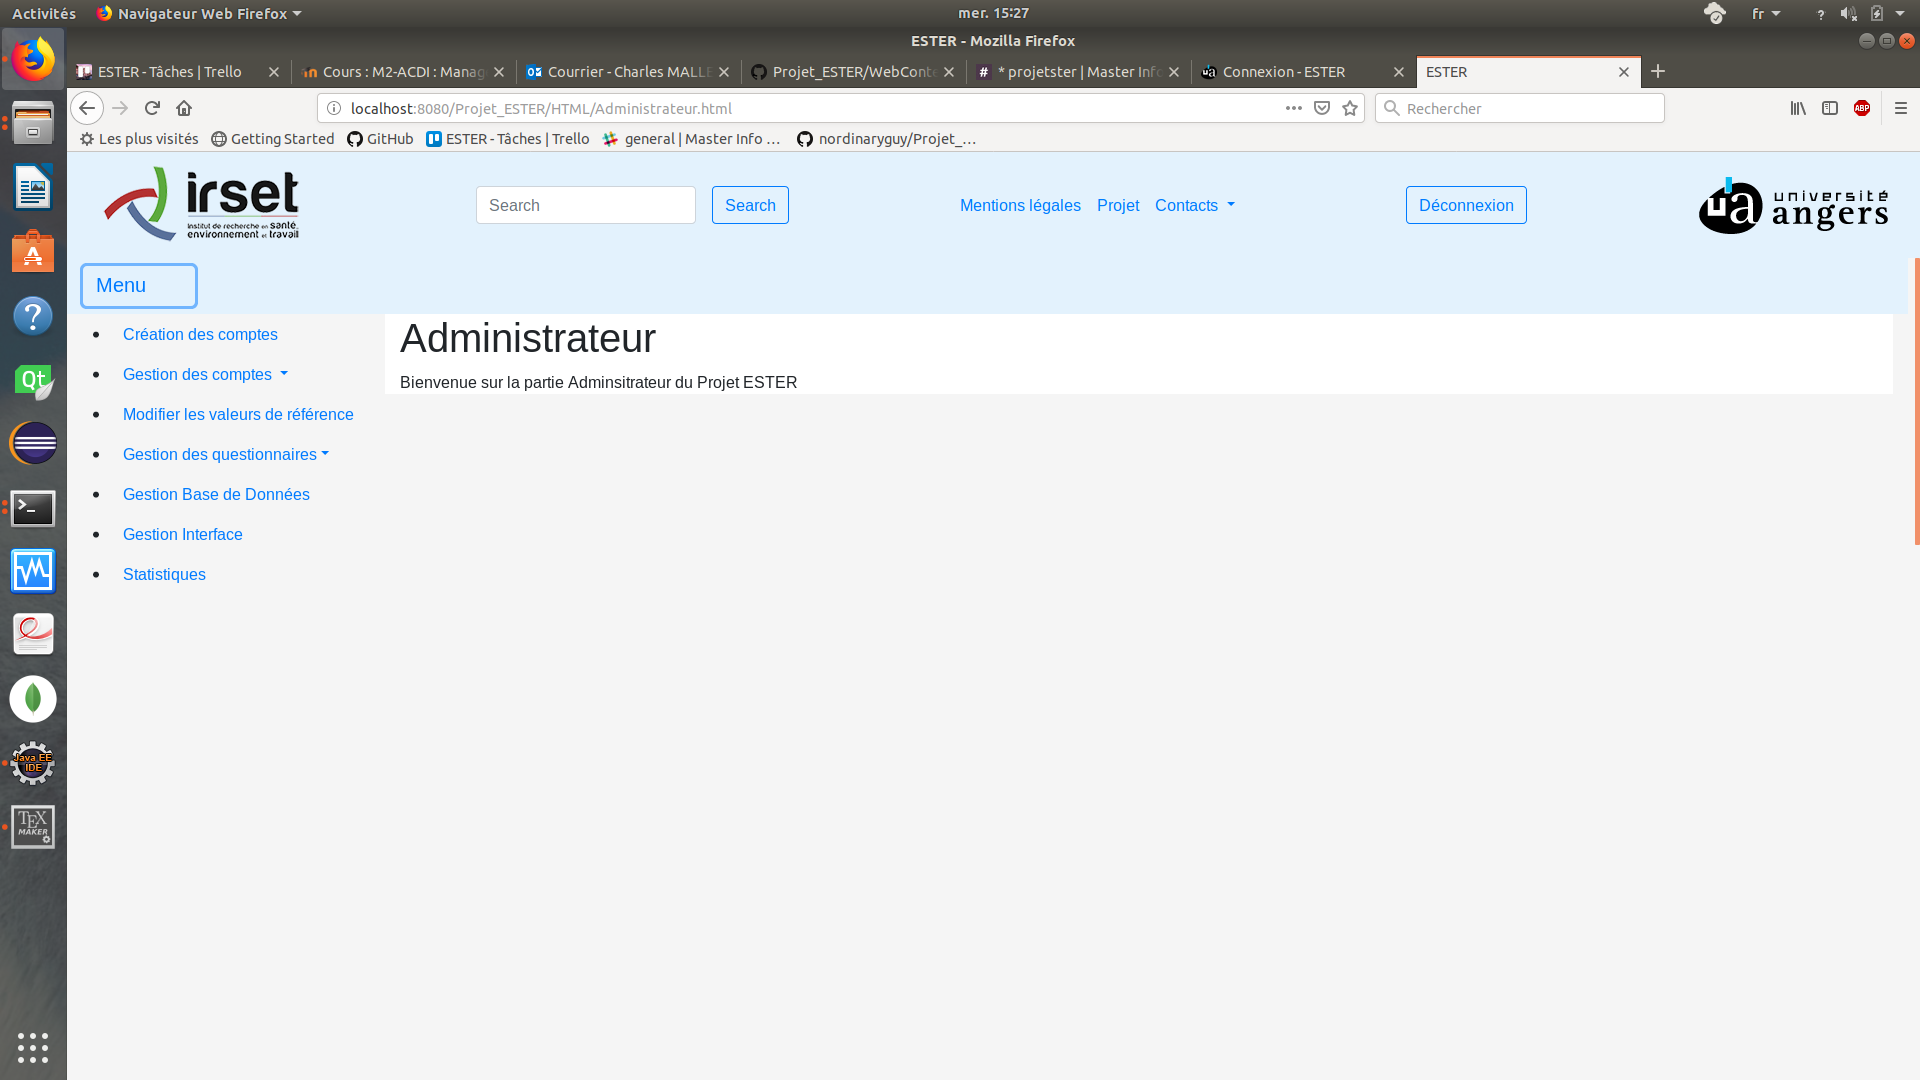
\includegraphics[scale=0.2,trim=2.8cm 0cm 0.8cm 5.3cm, clip=true]{img/OldAdmin}
    \end{center}
    \caption{Ancienne Page de l'Administrateur}
\end{figure}

Toutefois, les scripts HTML ont été remplacés par des script JSP permettant de rendre modulable le site tout entier : chaque page, selon un lien cliquable, peut afficher un nouveau champ et modifier des éléments du Back-end. Par ailleurs, nous avons défini deux fichiers JSP (un header et un footer) qui sont appelés dans la plupart de nos pages et qui servent aussi bien à se connecter qu'à se déplacer à travers le site, selon l'utilisateur connecté.

\begin{figure}[H]
    \begin{center}
	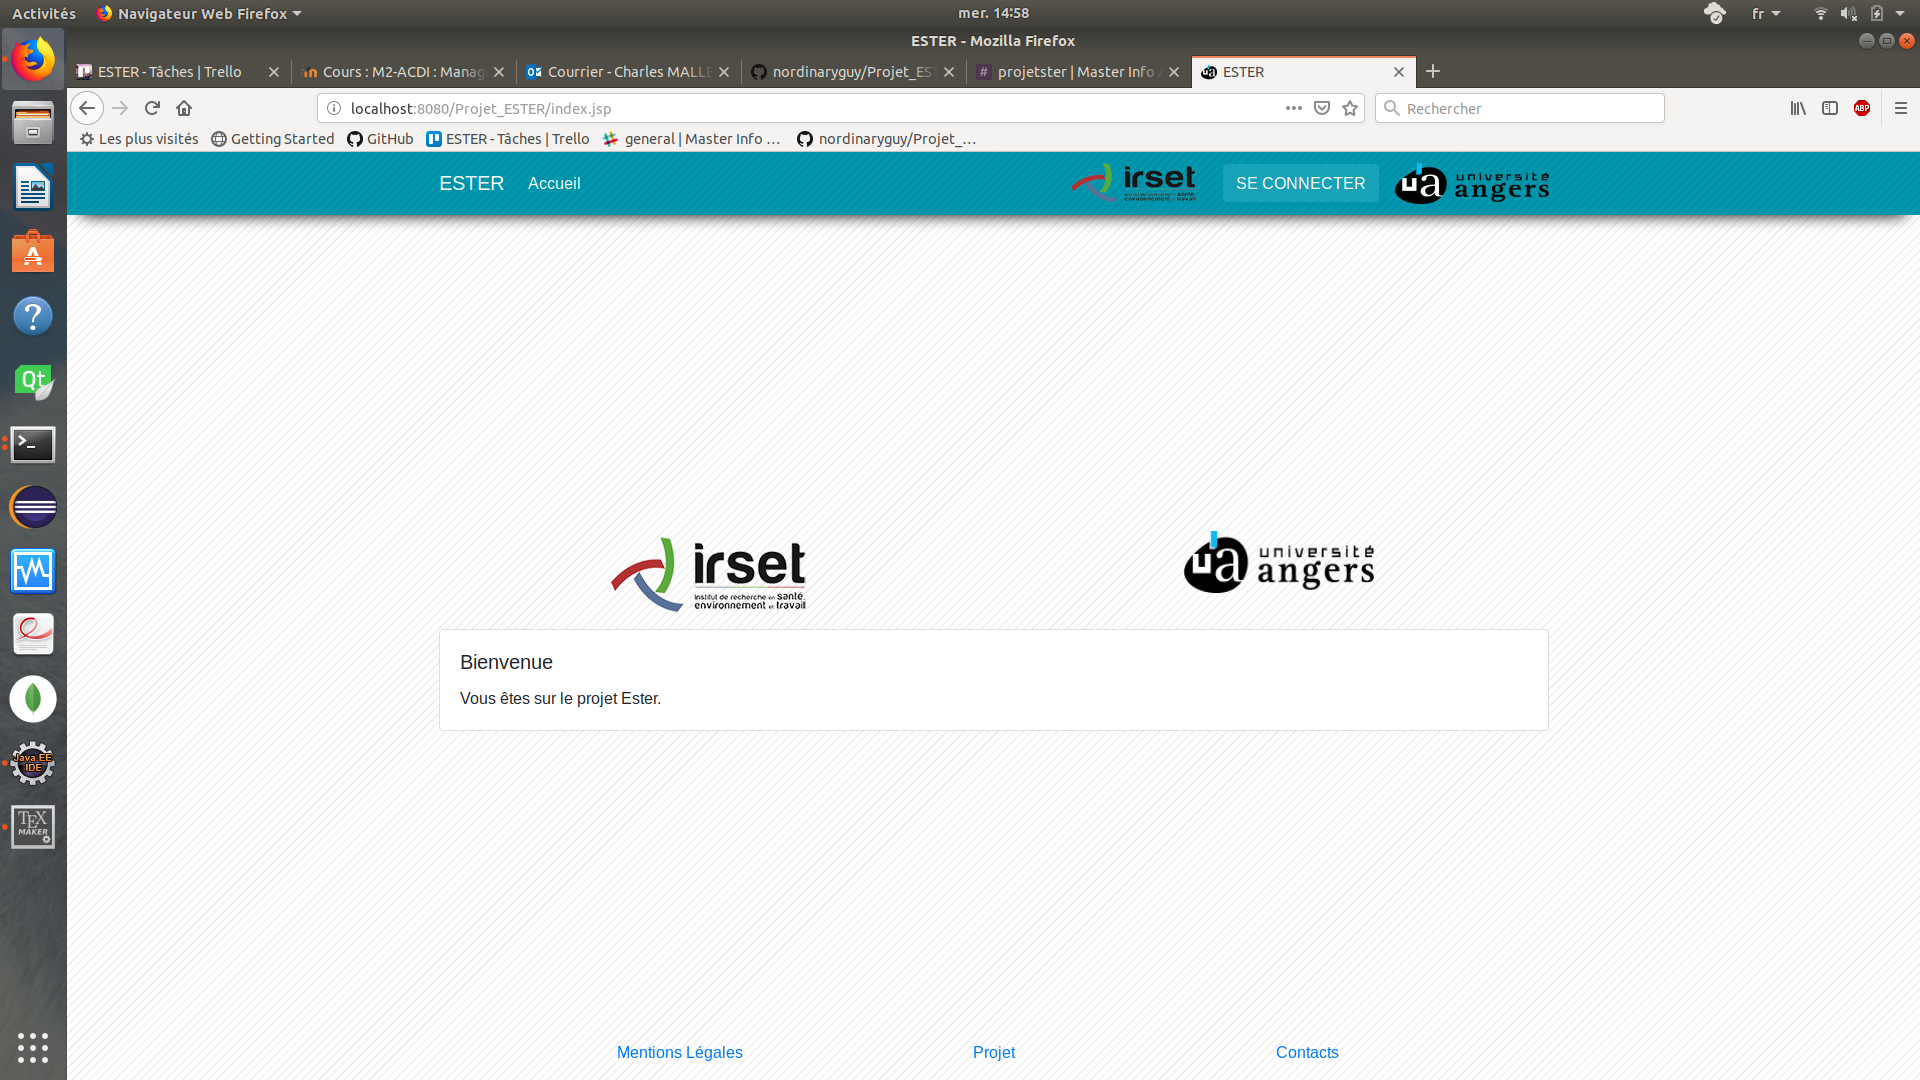
\includegraphics[scale=0.2,trim=4cm 0cm 4cm 5.3cm, clip=true]{img/ESTER}
    \end{center}
    \caption{Page d'Accueil ESTER}
\end{figure}

Afin de donner un exemple concernant l'aspect modulable de nos pages, nous pouvons regarder la page de Connexion. Sur cette dernière, en fonction du bouton sélectionné ("Salarié"/"Entreprise"/"Utilisateur" \footnote{Fait référence aux utilisateurs Médicaux et aux Administrateurs ; par opposition aux Entreprises et Salariés.}), vous aurez des champs de saisi différents. Puis, une fois la vérification effectuée, l'utilisateur du site sera redirigé automatiquement au bout de quelques secondes vers sa page.

\begin{figure}[H]
    \begin{center}
	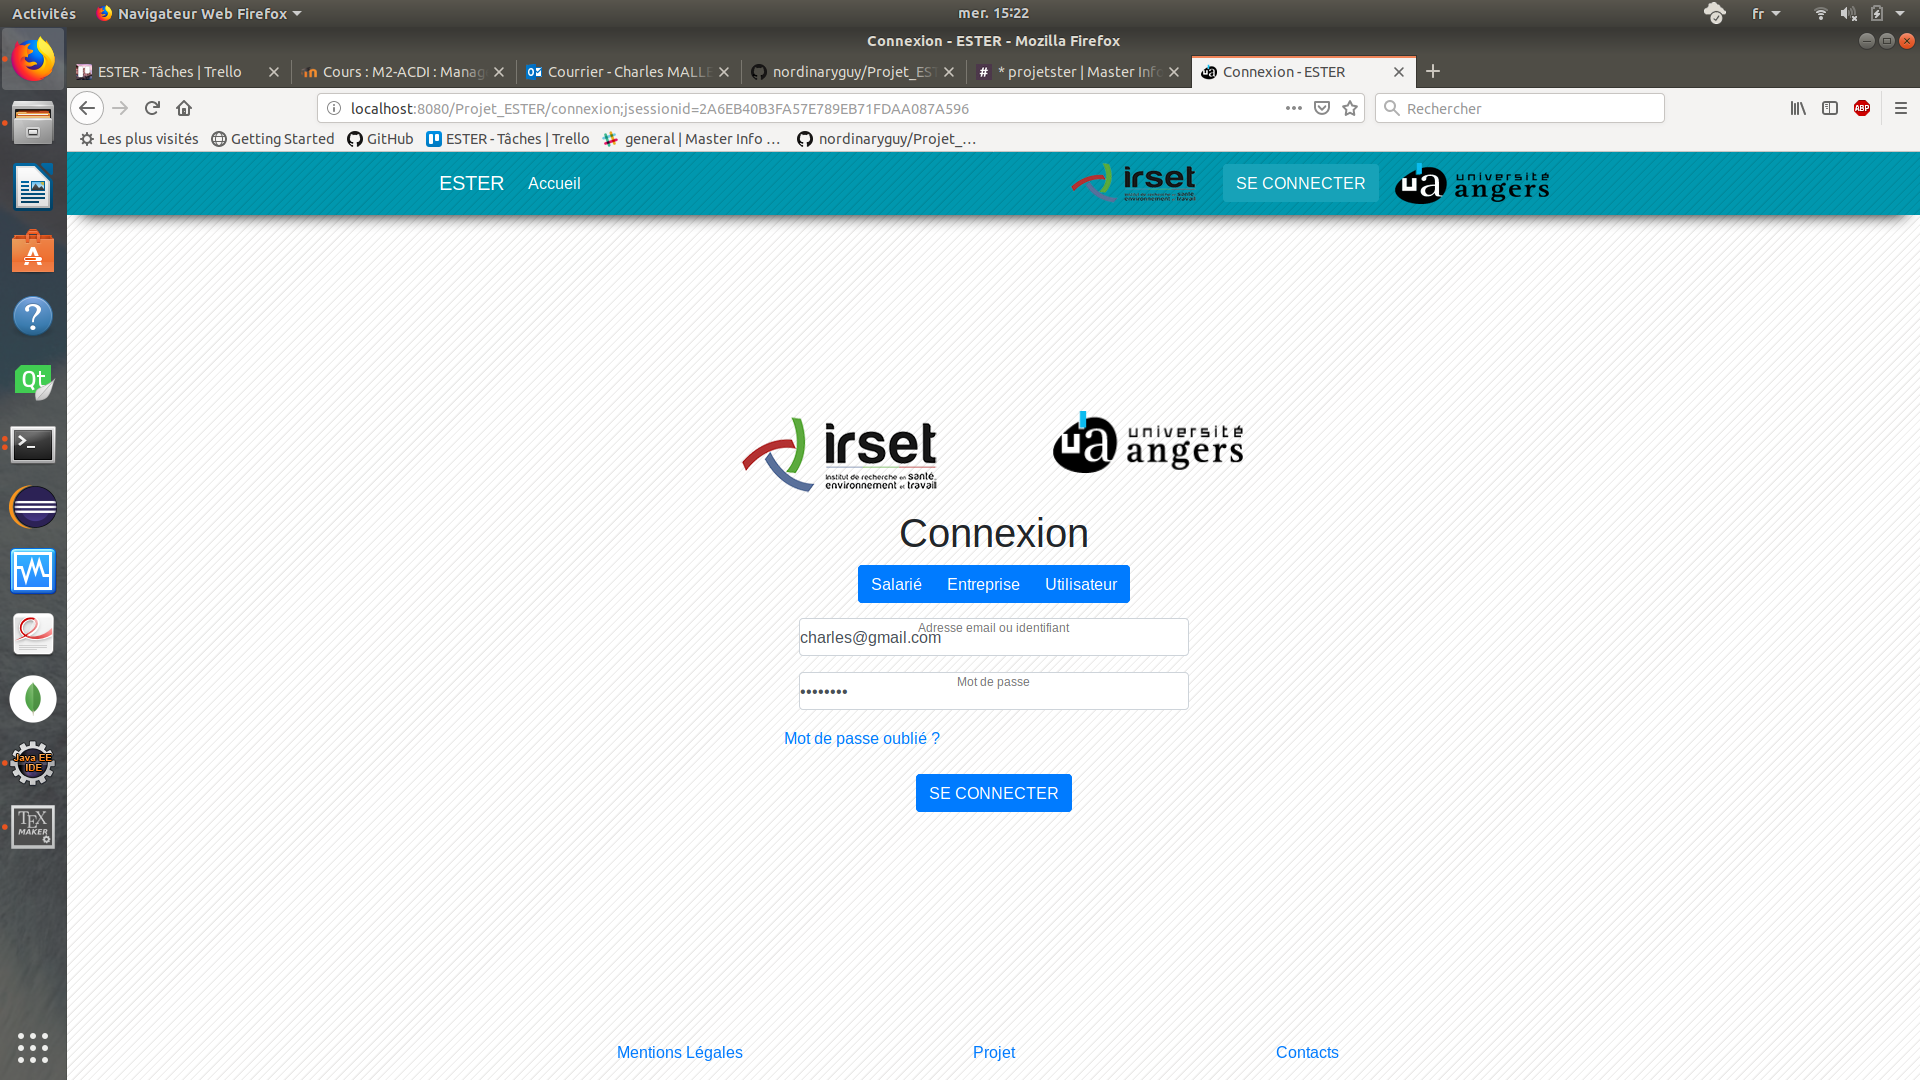
\includegraphics[scale=0.2,trim=4cm 0cm 4cm 5.3cm, clip=true]{img/Connexion}
    \end{center}
    \caption{Page de Connexion}
\end{figure}

Une fois connecté, l'utilisateur se retrouve sur la page qui correspond à son statut. Il peut choisir ce qu'il souhaite de faire en rapport des liens dans le Menu à gauche et pour certains liens, du contenu s'ajoutera sur sa page ou il sera redirigé vers une nouvelle page correspondante. 

\begin{figure}[H]
    \begin{center}
	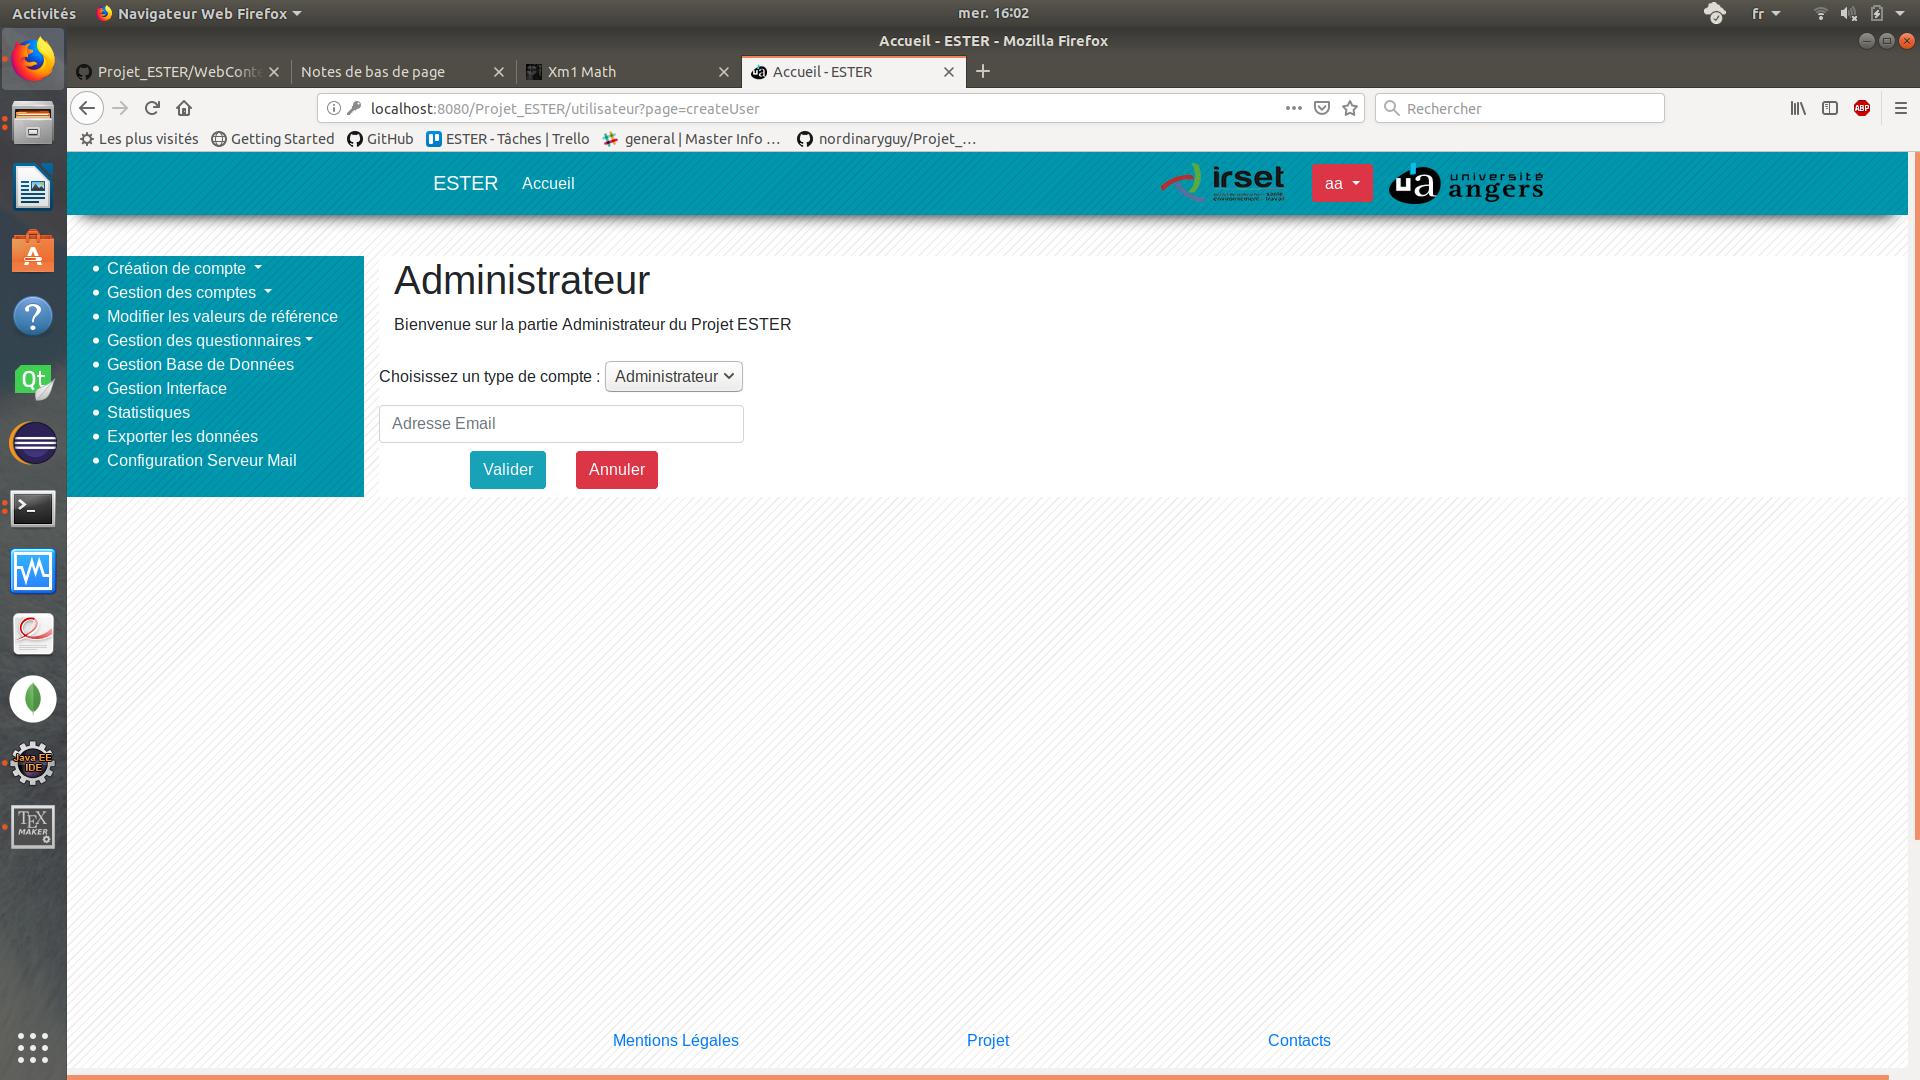
\includegraphics[scale=0.2,trim=2.8cm 0.1cm 0.8cm 5.3cm, clip=true]{img/Admin}
    \end{center}
    \caption{Page de l'Administrateur}
\end{figure}

